%=========================================================
\chapter{Modelo del Alcance}
\label{cap:reqUsr}

	En este capítulo se modela el alcance del sistema. Se presentan inicialmente los Actores involucrados y sus requerimientos, especificando cuales se alcanzaron en la primera iteración y cuales serán trabajados en la segunda iteración. Después se presentan los requerimientos funcionales de esta iteración y al final se presenta el modelo Físico y Lógico del sistema.


%---------------------------------------------------------


%---------------------------------------------------------
\section{Requerimientos}

\subsection{Requerimientos de Usuario}
	\begin{requerimientosU}
		\FUitem{RU1}{Conocer info de profesores}{Los      padres de familia deben poder visualizar la
            informacion de los profesores en el momento que lo requieran}{Alta}
		\FUitem{RU2}{Registro de niños}{Los profesores deben poder seleccionar a los niños para realizar el reporte de estos.}{Alta}
		\FUitem{RU3}{Registro de salas}{Se necesita poder asignar a los niños a las salas, visualizando la disponibilidad de las salas.}{Moderada}
		\FUitem{RU4}{Registro de menú}{Se necesita tener el registro de lo que los niños van a comer durante el mes, y que los padres lo puedan visualizar}{baja}
		\FUitem{RU5}{Registro de ingestas}{Se necesita tener registro de que tanto comieron los niños para que los padres puedan visualizarlo.}{Moderada}
            \FUitem{RU6}{Registro de evacuaciones}{Se necesita tener registro de las evacuaciones los niños para que los padres puedan visualizarlo.}{Moderada}
            \FUitem{RU7}{Registro de actividades}{Se necesita tener registro de las actividades realizadas por los niños para que los padres puedan visualizarlo.}{Baja}
            \FUitem{RU8}{Registro de actividades en casa}{Los profesores necesitan poder registrar las actividades que los niños tienen que hacer en casa para que los padres puedan enterarse.}{Baja}
            \FUitem{RU9}{Incidencias médicas}{Se necesita tener un registro de cada diagnostico que el doctor le realiza a un niño.}{Moderada}
            \FUitem{RU10}{Solicitud de material}{Los profesores necesitan registrar los materiales que se ocuparán en cada clase.}{Baja}
            \FUitem{RU11}{Eventos escolares}{La directora necesita registrar cuándo hay eventos escolares.}{Moderada}
            \FUitem{RU12}{Dias inhabiles}{La directora necesita registrar los días inhábiles.}{Baja}
            \FUitem{RU13}{Asistencia}{Se necesita registrar la asistencia de cada niño en cada grupo por su profesor.}{Moderada}
            \FUitem{RU14}{Cambios de ropa}{Los profesores necesitan registrar los cambios de ropa de los niños durante el día.}{Moderada}
            \FUitem{RU15}{Reportes}{En caso de alguna incidencia con alguno de los niños, el profesor debe hacer un reporte sobre lo ocurrido, se tiene que llevar un registro de estos reportes.}{Moderada}
            \FUitem{RU16}{Citas}{Los profezores y doctores necesitan agendar citas con los tutores responsables de cada niño.}{Baja}
            \FUitem{RU17}{Modificacion info-niños}{Capital Humano necesita poder modificar cualquier informacion de los niños inscritos a la guarderia en cualquier momento.}{Alta}
            \FUitem{RU18}{Modificacion info-profesores}{Recursos Humanos necesita poder modificar la informacion del personal de la guarderia en cualquier momento de forma rapida.}{Alta}
            \FUitem{RU19}{Permisos y autorizaciones}{Los padres necesitan dar de alta a dos personas mas responsables del niño, en caso de que ellos no puedan recoger al niño}{Alta}
            \FUitem{RU20}{Escalabilidad de usuarios}{El personal de la guarderia necesita consultar rapidamente la informacion de los niños, asi como la informacion de cualquier otro personal.}{Alta}
            \FUitem{RU21}{Asignacion de alumnos a salas}{Capital Humanos necesita asignar a cada niño a su grupo y salon correspondiente}{Moderada}
            \FUitem{RU22}{Asignar profesores a salas}{La guarderia necesita por cada salon a un profesor y dos auxiliares}{Moderada}
            \FUitem{RU23}{Acceso 24/7 a los reportes de los alumnos}{Se rquiere reformar la forma en la que los tutores acceden a los reportes de sus hijos, pudiendo ahora acceder en cualquier momento de la semana, sin restricciones horarias.}{Alta}
            
            \FUitem{RU24}{Acceso a los reportes}{Se mantendrá el acceso exclusivo de los padres a los reportes de sus hijos, sin la capacidad de realizar acciones de personal administrativo.}{Alta}
            \FUitem{RU25}{Sitio web}{La plataforma debe ser una página web con un diseño moderno, intuitivo y fácil de navegar para el usuario.}{Alta}
            \FUitem{RU26}{Registro padres}{El personal de servicios sociales llevara a cabo el registro de tutores de los ninos, este registro se realizara cada periodo de inscripciones/reinscripciones.}{Alta}
            \FUitem{Ru27}{Fotografias}{Se debe mantener el sistema actual de identificacion de ninos y tutores, por lo que se requiere guardar una fotografía de cada uno para su facil identificacion.}{Moderada}
            \FUitem{RU28}{Seguridad}{Se deben tomar medidas de seguridad para garantizar que la información de los padres y alumnos esté protegida contra accesos no autorizados o fugas de información.}{Moderada}
            \FUitem{RU29}{Interfaz de usuario facil de usar}{La plataforma debe ser fácil de usar, con una interfaz intuitiva que permita a cualquier usuario acceder a la información correspondiente de manera sencilla.}{Baja}
            \FUitem{RU30}{Estudio socioeconomico}{Se requerirá que los padres respondan unas preguntas simples para conocer su situación económica, sin la necesidad de completar formularios complejos o extensos.}{Baja}
	\end{requerimientosU}
    


%---------------------------------------------------------
\subsection{Requerimientos funcionales}
    \begin{requerimientos}
        \FRitem{RF1}{Registro profesores}{Recursos Humanos deberá ingresar el nombre, dirección, número de teléfono.}{Alta}{RU1}
        \FRitem{RF2}{Creacion usuario y contraseña profesor}{Una vez registrados los datos del profesor, el sistema le asignará un usuario y contraseña para que el profesor pueda acceder a las funciones de los profesores.}{Alta}{RU1}
        \FRitem{RF3}{Cambiar contraseña profesor}{El profesor podrá cambiar su contraseña ingresando la contraseña actual y su nueva contraseña.}{Alta}{RU1}
        \FRitem{RF4}{registro padres}{Capital humano deberá ingresar el nombre, dirección, número de teléfono.}{Alta}{RU26}
        \FRitem{RF5}{Creacion usuario y contraseña padre}{Una vez registrados los datos del profesor, el sistema le asignará un usuario y contraseña para que el profesor pueda acceder a las funciones de los padres.}{Alta}{RU26}
        \FRitem{RF6}{Cambiar contraseña padre}{El padre podrá cambiar su contraseña ingresando la contraseña actual y su nueva contraseña.}{Alta}{RU26}
        \FRitem{RF7}{Inicio sesion profesor}{Los profesores ingresarán su usuario y contraseña, entonces el sistema validará la existencia de ese usuario y de ser que exista, le otorgara su token de acceso. }{Moderada}{RU28}
        \FRitem{RF8}{Inicio sesion padre}{Los padres ingresarán su usuario y contraseña, entonces el sistema validará la existencia de ese usuario y de ser que exista, le otorgara su token de acceso.}{Moderada}{RU28}
        \FRitem{RF9}{Registro niños}{Capital humano deberá ingresar el nombre, dirección, edad.}{Alta}{RU2}
        \FRitem{RF10}{Enlazar padre-niño}{Capital humano asignará a cada padre de familia los niños de los que es \textquotedblleft responsable\textquotedblright .}{Alta}{RU19}
        \FRitem{RF11}{Registro salas}{Capital humano deberá ingresar el nombre, grado, y localización de una sala.}{Moderada}{RU3}
        \FRitem{RF12}{Registro nutriologo}{Capital humano deberá ingresar el nombre, dirección, cédula del nutriologo.}{Baja}{RU4}
        \FRitem{RF13}{Usuario y contraseña nutriologo}{Una vez registrados los datos del nutriólogo, el sistema le asignará un usuario y contraseña para que el profesor pueda acceder a las funciones del nutriólogo.}{Baja}{RU4}
        \FRitem{RF14}{Inicio sesión nutriologo}{El nutriólogo ingresará su usuario y contraseña, entonces el sistema validará la existencia de ese usuario y de ser que exista, le otorgara su token de acceso.}{Baja}{RU4}
        \FRitem{RF15}{Registro menú}{El nutriólogo ingresará las comidas de cada día hábil.}{Baja}{RU4}
        \FRitem{RF16}{Visualizacion menú mensual}{Los padres de familia podrán visualizar el menú del mes actual.}{Baja}{RU4}
        \FRitem{RF17}{Vsualizacion menú del día}{Al momento de que los padres de familia ingresen al sistema, se les mostrara el menú planeado para el dia actual.}{Baja}{RU4}
        \FRitem{RF18}{Viusalizacion menú día especifico}{Los padres de familia podrán seleccionar un dia del mes actual o de un mes pasado y visualizar el menú de ese dia.}{Baja}{RU4}
        \FRitem{RF19}{Registro de ingestas}{Los profesores podran seleccionar una sala y podran seleccionar uno de las opciones de ingesta de cada niño para cada comida.}{Alta}{RU5}
        \FRitem{RF20}{Registro de evacuaciones}{Los profesores podran seleccionar una sala y podran seleccionar uno de las opciones de evacuacion de cada niño y la cantidad de estas.}{Alta}{RU6}
        \FRitem{RF21}{Registro actividadees}{Los profesores podran seleccionar una sala y registrar que actividades realizaron con esa sala en el dia actual.}{Alta}{RU7}
        \FRitem{RF22}{Registro de actividades en casa}{Los profesores podran seleccionar una sala y registrar que actividades tienen que hacer los niños en sus casas.}{Alta}{RU8}
        \FRitem{RF23}{Visualizacion de actividades en casa}{Al entrar al sistema, los padres podran ver que actividades tienen que hacer con sus hijos para el siguiente dia.}{Alta}{RU8}
        \FRitem{RF24}{Registro medico}{Capital humano ingresará el nombre, dirección, telefono, cedula del médico.}{Alta}{RU9}
        \FRitem{RF25}{Asignacion usuario y contraseña medico}{Una vez registrados los datos del médico, el sistema le asignará un usuario y contraseña para que el profesor pueda acceder a las funciones del médico.}{Moderada}{RU9}
        \FRitem{RF26}{Inicio sesión medico}{El médico ingresará su usuario y contraseña, entonces el sistema validará la existencia de ese usuario y de ser que exista, le otorgara su token de acceso.}{Moderada}{RU9}
        \FRitem{RF27}{Registro incidencia medica}{El médico seleccionará a un niño y registrara la fecha y hora del incidente así como el incidente en si.}{Baja}{RU9}
        \FRitem{RF28}{Solicitud material}{Los profesores registraron el material que necesitan para la siguiente clase}{Baja}{RU10}
        \FRitem{RF29}{Visualización material}{Cuando los padres de familia accedan al sistema, se les mostrará un aviso con el material que deben de llevar para el siguiente día.}{Baja}{RU10}
        \FRitem{RF30}{Registro de eventos escolares}{El director seleccionará una fecha y registrará un evento para ese dia, ademas de la hora de inicio y fin del evento.}{Alta}{RU11}
        \FRitem{RF31}{Inicio sesión director}{El director ingresará su usuario y contraseña, entonces el sistema validará la existencia de ese usuario y de ser que exista, le otorgara su token de acceso.}{Alta}{RU11}
        \FRitem{RF32}{Visualización de eventos escolares}{El sistema contará con una sección de próximas fechas donde se mostrarán los siguientes eventos escolares.}{Alta}{RU11}
        \FRitem{RF33}{Detalle eventos escolares}{Los padres de familia podrán seleccionar un evento escolar de la sección de próximas fechas y visualiza los detalles del evento.}{Media}{RU11}
        \FRitem{RF34}{Registro de días inhabiles}{El director seleccionará una fecha y lo marcará como dia habil.}{Baja}{RU12}
        \FRitem{RF35}{Visualizacion días inhabiles}{El sistema contara con una sección de fechas importantes donde se mostraran los días inhábiles.}{Alta}{RU12}
        \FRitem{RF36}{Toma de asistencia}{El profesor podrá consultar una lista con todos los niños de sus salas asignadas y marcará que niños asistieron y a que hora ingresaron.}{Alta}{RU13}
        \FRitem{RF37}{Registrar salida}{El profesor podrá consultar una lista con todos los niños que se encuentran en su sala seleccionara uno y registrara su hora de salida.}{Alta}{RU13}
        \FRitem{RF38}{Registrar cambio de ropa}{El profesor registrará la ropa que los padres le entregan y a que niño le pertenece.}{Baja}{RU14}
        \FRitem{RF39}{Consulta ropa}{El sistema le mostrará al profesor cuantas mudas tiene un niño y el estado de estas mudas, mostrando un aviso cuando no queden mudas limpias.}{Baja}{RU14}
        \FRitem{RF40}{Registrar uso de ropa}{El profesor registrará el uso de una muda de ropa y el sistema removerá esa muda de la lista de mudas disponibles.}{Baja}{RU14}
        \FRitem{RF41}{Generar reporte diario infante}{El sistema generará un reporte de cada niño con la fecha del reporte, las ingestas del niño, sus evacuaciones, su hora de entrada y su hora de salida.}{Alta}{RU15}
        \FRitem{RF42}{Registro informacion adicional al reporte diario infante}{El profesor podrá seleccionar a un niño que pertenezca a una de sus salas asignadas y le registrara observaciones para incluirlo en el reporte diario.}{Moderada}{RU15}
        \FRitem{RF43}{Visualizar reporte}{Los padres de familia podrán seleccionar a uno de sus niños y veran el reporte diario del niño.}{Moderado}{RU15}
        \FRitem{RF44}{Generar cita con un padre}{El profesor seleccionará a un niño, una fecha y hora para solicitar un citatorio con algún encargado del niño.}{Baja}{RU16}
        \FRitem{RF45}{Medico solicita cita}{El médico seleccionará a un niño, una fecha y hora para solicitar un citatorio con algún encargado del niño}{Baja}{RU16}
        \FRitem{RF46}{Generar cita con profesor}{Los padres de familia seleccionarán una fecha y hora para solicitar un citatorio con los profesores asignados a la sala de uno de sus niños.}{Baja}{RU16}
        \FRitem{RF47}{Generar cita con medico}{Los padres de familia seleccionarán una fecha y hora para solicitar un citatorio con el médico.}{Baja}{RU16}
        \FRitem{RF48}{Visualizar cita padre}{El sistema contará con el apartado de citatorios, donde los padres de familia podrán visualizar todos los citatorios que han solicitado y todos los citatorios a los que le citaron.}{Baja}{RU16}
        \FRitem{RF49}{Visualizar cita profesor}{El sistema contará con el apartado de citatorios, donde los profesores podrán visualizar todos los citatorios que han solicitado y todos los citatorios a los que le citaron.}{Baja}{RU16}
        \FRitem{RF50}{Visualizar cita medico}{El sistema contará con el apartado de citatorios, donde los médicos podrán visualizar todos los citatorios que han solicitado y todos los citatorios a los que le citaron.}{Baja}{RU16}
        \FRitem{RF51}{Modificar datos infante}{Capital humano podrá actualizar los datos de los niños.}{Baja}{RU17}
    \end{requerimientos}


%---------------------------------------------------------
\subsection{Requerimientos no funcionales}
    \subsubsection{Requerimientos del negocio}
    \begin{NFRequerimientos}
        \NFRitem{RNF1}{Colores del establecimiento}{Los colores de las pantallas deberán ser los colores que usa.}{Alta}{RU25}
        \NFRitem{RNF2}{Roles dentro del negocio}{Al igual de en la guardería, existe una distribución en las personas encargadas en cada área del trabajo, y cada área se encarga de una tarea en específico.}{Alta}{RU1, RU2, RU3, RU4, RU5}
        \NFRitem{RNF3}{Niños en grupos especificos}{Un grupo de niños no puede tener más de 30 niños y se dividen en grupos por edad (Lactantes de 3 meses a 1 año, 1 - 2 años y Maternal hasta los 6 años)}{Alta}{RU3}
        \NFRitem{RNF4}{Menú guarderia}{El nutriólogo da hasta 4 menús diarios distintos y estos llegan a depender de notas hechas por los padres sobre el niño.}{Alta}{RU4}
        \NFRitem{RNF5}{Reporte de incidencias médicas}{El doctor no puede hacer recetas médicas, pero sí observaciones y evalúa al niño en cuanto surja un incidente y tiene que notificarle al tutor.}{Alta}{RU9}
        \NFRitem{RNF6}{Niños especiales}{Es posible aceptar a niños especiales dentro de la guardería, siempre y cuando toda su información correspondiente sea notificada antes de hacer su inscripción.}{Alta}{RU2}
        \NFRitem{RNF7}{Seguridad en el establecimiento}{Existen medidas implementadas para identificar correctamente a los niños con sus tutores y esto es mediante credenciales y conociendo una foto del tutor responsable que debe estar dentro del sistema.}{Alta}{RU7}
        \NFRitem{RNF8}{Horario de la guarderia}{No existe un tiempo definido para que los profesores escriban los reportes a los niños correspondientes.}{Moderada}{RU8}
        \NFRitem{RNF9}{Evaluacion y seguimiento del desarrollo del niño}{Se realizarán evaluaciones periódicas del desarrollo de los niños para identificar posibles problemas y garantizar que estén recibiendo la atención necesaria.}{Moderada}{RU6}
        \NFRitem{RNF10}{Comunicación con los padres}{Se mantendrá una comunicación constante con los padres, por medio de reuniones periódicas, para informarles sobre el desarrollo de sus hijos y cualquier incidente que surja en la guardería, ademas de avisos dentro del sistema.}{Moderada}{RU10}
        \NFRitem{RNF11}{Profesores encargados}{En cada sala debe haber tres profesores por turno asignados para cuidar al grupo.}{Baja}{RU1}
        \NFRitem{RNF12}{Profesores por turno}{La guardería cuenta con dos turnos, por lo que al cambio de turno, cambian los profesores a cargo del grupo.}{Baja}{RU1}
        \NFRitem{RNF13}{Encargados alumno}{cada niño es asignado a su padre de familia mas dos encargados que pueden pasar a recogerlo.}{Baja}{RU26}
        \end{NFRequerimientos}

        \subsubsection{Requerimientos de informacion y datos}
        \begin{NFRequerimientos}
        \NFRitem{RNF14}{Seguridad en almacenamiento de la informacion}{Debe ser un sistema seguro para mantener la información privada tanto de las personal de la guardería, como de los clientes.}{Alta}{RU28}
        \NFRitem{RNF15}{Seguridad en el acceso a la informacion}{No todos los miembros del personal tienen acceso a los mismos datos de los clientes.}{Alta}{RU28}
        \NFRitem{RNF16}{Seguridad de contraseñas}{Las contraseñas deben ser cifradas, dentro del sistema para que solamente los clientes de las guarderías puedan entrar.}{Moderada}{RU28}
        \NFRitem{RNF17}{Informacion correspondiente}{La información del cliente debe corresponder a solamente a él, y debe ser inaccesible para terceros.}{Alta}{RU28}
        \NFRitem{RNF18}{Almacenamiento}{Toda la información agregada al sistema debe poder ser guardada por más de 6 años, en el transcurso del tiempo puede ser modificada o alterada.}{Alta}{RU23}
        \NFRitem{RNF19}{Cedulas profesionales}{La cedula profesional de los profesores y de los doctores y nutriologas puede ser vista dentro de la página de la guardería para todos los tutores que esten en la guarderia.}{Baja}{RU1, RU9}
        \NFRitem{RNF20}{Copias de seguridad periodicas}{El sistema debe realizar copias de seguridad periódicas, para garantizar la disponibilidad de la información en caso de pérdida o daño al sistema.}{Alta}{RU23}
        \NFRitem{RNF21}{Registro de accesos y cambios}{El sistema debe llevar un registro de accesos y cambios realizados en la información para garantizar la trazabilidad y la seguridad de la información.}{Alta}{RU23, RU28}
        \NFRitem{RNF22}{Seguridad}{El sistema debe contar con medidas de seguridad para proteger la información de los usuarios y el acceso no autorizado a la plataforma.}{Alta}{RU28}
        \NFRitem{RNF23}{Pruebas de seguridad}{El sistema debe someterse periódicamente a pruebas de seguridad para detectar posibles fallos o vulnerabilidades en su funcionamiento.}{Moderada}{RU28}
        \NFRitem{RNF24}{Privacidad de datos}{El sistema debe respetar la privacidad de los datos de los usuarios y cumplir con las leyes de protección de datos personales.}{Alta}{RU28}
        \NFRitem{RNF25}{Actualizacion de software}{El sistema debe actualizar regularmente su software y parches de seguridad para garantizar la protección y seguridad de la información.}{Alta}{RU23, RU28}
        \NFRitem{RNF26}{Formato contraseña}{Las contraseñas deben de contener al menos una mayúscula, una minúscula y un número, además de tener una extensión de mínima de 8 caracteres.}{Baja}{RU28}
        \NFRitem{RNF27}{Manejo de tokens}{El sistema manejara tokens para controlar el acceso y estos se desactivarán después de un lapso de inactividad de 5 minutos.}{Baja}{RU28}
        \end{NFRequerimientos}


        \subsubsection{Requerimientos de interaccion con el usuario}
        \begin{NFRequerimientos}
        \NFRitem{RNF28}{Tiempo de acceso}{No debe de tomarle más de 5 segundos al usuario ingresar a su cuenta.}{Baja}{RU23}
        \NFRitem{RNF29}{Tiempo de interaccion}{No debera de tardar más de 5 segundos el usuario en hacer o recibir una solicitud de la página.}{Baja}{RU23}
        \NFRitem{RNF30}{Capacidad de respuesta}{El sistema debe responder de manera rápida y sin demora ante las acciones del usuario.}{Moderada}{RU20, RU23}
        \NFRitem{RNF31}{Disponibilidad con usuarios}{La aplicación debe estar disponible en todo momento, salvo en mantenimientos planificados.}{Alta}{RU1}
        \NFRitem{RNF32}{Accesibilidad de usuarios}{La aplicación debe ser accesible para todos los usuarios, incluyendo personas con discapacidades, mediante el uso de tecnologías de apoyo.}{Alta}{RU12}
        \NFRitem{RNF33}{Estabilidad de usuarios}{La aplicación debe ser estable y no presentar errores críticos que afecten su funcionamiento.}{Alta}{RU1, RU20, RU23}
        \NFRitem{RNF34}{Valores}{Todas las paginas deben estar escritas correctamente con respeto a los usuarios}{Baja}{RU1}
        \NFRitem{RNF35}{Mensajes limitantes}{Los usuarios pueden mandar mensajes directos a subdirección si tienen dudas específicas.}{Baja}{RU1}
        \NFRitem{RNF36}{Notificaciones}{Las notificaciones deben llegar al correo electronico de los tutores y al celular como un mensaje.}{Baja}{RU1, RU20, RU23}
        \NFRitem{RNF37}{Tipos salidas}{La salida de datos debe ser visualizada en una pantalla.}{Alta}{RU1}
        \NFRitem{RNF38}{Inputs}{La aplicación debe funcionar sin nuevos dispositivos de entrada, mas que el teclado y mouse.}{Alta}{RU1}
        \end{NFRequerimientos}

        \subsubsection{Requerimientos de plataforma}
        \begin{NFRequerimientos}
        \NFRitem{RNF39}{Plataforma del sistema}{El sistema debe ser capaz de correr desde una computadora en un navegador web, como en un celular.}{Alta}{RU23}
        \NFRitem{RNF40}{Escalabilidad dentro del sistema}{El sistema debe tener la capacidad de ir creciendo, conforme crece el negocio.}{Alta}{RU20}
        \NFRitem{RNF41}{Disponibilidad del sistema}{El sistema debe estar disponible las 24 horas del día todos los días de la semana, en caso de hacer mantenimiento este no deberá dejar el servicio por máximo 30 minutos.}{Alta}{RU23}
        \NFRitem{RNF42}{Integración con otras herramientas}{El sistema debe poder integrarse con otras herramientas o software utilizados por la organización, para mejorar el flujo de trabajo y la eficiencia del negocio.}{Moderada}{RU19}
        \NFRitem{RNF43}{Escalabilidad en la base de datos}{La base de datos del sistema debe ser escalable para soportar un gran volumen de datos sin perder rendimiento.}{Moderada}{RU20}
        \NFRitem{RNF44}{Interfaz del usuario intuitiva}{La interfaz de usuario del sistema debe ser fácil de usar y entender para cualquier tipo de usuario.}{Moderada}{RU22}
        \NFRitem{RNF45}{Compatibilidad con diferentes navegadores}{El sistema debe ser compatible con los navegadores más utilizados como Chrome, Firefox, Safari y Edge.}{Moderada}{RU23}
        \NFRitem{RNF46}{Capacidad de exportar datos}{El sistema debe permitir la exportación de datos en diferentes formatos para realizar análisis externos y generar informes personalizados.}{Moderada}{RU21}
        \NFRitem{RNF47}{Multidispositivo}{La aplicación debe ser compatible y adaptarse a diferentes dispositivos, como ordenadores, smartphones y tablets.}{Alta}{RU14}
        \end{NFRequerimientos}

        \subsubsection{Requerimientos de propiedades de software}
        \begin{NFRequerimientos}
        \NFRitem{RNF48}{Sistema amigable}{Debe ser fácil para los usuarios interactuar con el sistema, y que les parezca intuitivo manejarlo.}{Baja}{RU29}
        \NFRitem{RNF49}{Calidad dentro del proyecto}{Debe ser atractivo visualmente todas las páginas del sistema.}{Baja}{RU29}
        \NFRitem{RNF50}{Confiabilidad}{El sistema debe estar libre de bugs o errores al momento de ser desplegado para no interferir con la experiencia del usuario.}{Alta}{RU29}
        \NFRitem{RNF51}{Mantenibilidad}{El sistema puede ser modificado dentro del tiempo que es usado, por decisión de los stakeholders, además de que pueda ser transparente(Ningún cambio afecte el funcionamiento del sistema ni de su información ya almacenada).}{Moderada}{RU25}
        \NFRitem{RNF52}{Estabilidad}{No puede caerse el sistema si hay una gran cantidad de usuarios activos en el momento de operación, ni afectar su desempeño.}{Moderada}{RU20}
        \NFRitem{RNF53}{Privacidad}{Debe de mantenerse privada la información personal de todos los usuarios ante terceros, además solo la podrán ver personal específico de la guardería.}{Alta}{RU28}
        \NFRitem{RNF54}{Seguridad}{El sistema debe contar con medidas de seguridad para proteger la información almacenada en él, como cifrado de datos y autenticación de usuarios.}{Alta}{RU28}
        \NFRitem{RNF55}{Escalabilidad}{El sistema debe ser capaz de crecer y aumentar su capacidad de manejo de usuarios e información de manera eficiente y sin comprometer su rendimiento.}{Moderada}{RU20}
        \NFRitem{RNF56}{Documentacion}{El sistema debe contar con una documentación adecuada que permita comprender su funcionamiento y facilitar su mantenimiento por parte de los desarrolladores.}{Baja}{RU25}
        \NFRitem{RNF57}{Tamaño fotos}{El sistema redimensiona las fotos de los encargados de los niños a 500 px x 400px.}{Baja}{RU27}
        \NFRitem{RNF58}{Responsivo}{La página web del sistema debe de ser responsiva.}{Baja}{RU29}
        \NFRitem{RNF59}{Host}{El sistema debe estar hosteado en un dominio .com}{Baja}{RU25}
        \NFRitem{RNF60}{BD}{La base de datos de datos debe de estar hosteada en un servidor.}{Baja}{RU25}
        
    \end{NFRequerimientos}

    
%---------------------------------------------------------
\section{Especificación de plataforma}	
	
\begin{description}
	\item[Tipo de sistema:] Nuestro sistema se implementara con una aplicación web.
	\item[Software requerido:] Para el funcionamiento de la aplicacion web se requiere lo siguiente:
        \begin{itemize}
            \item {\bf Sistema operativo}:Compatible con Windows, macOS y Linux
            \item {\bf Navegador web}:
            \item {\bf Servidor}:
            \item {\bf Lenguajes de programacion}:
            \item {\bf Frameworks}:
            \item {\bf Base de datos}:
            \item {\bf IDE}: Se recomienda el uso de Visual Studio Code para el desarrollo
        \end{itemize}
	\item[Hardware requerido:] Para un renimiento optimo se recomienda el siguiente hardware
        \begin{itemize}
            \item {\bf CPU}:Intel core i5 8th Gen o equivalente
            \item {\bf Memoria RAM}:Minimo 4 GB
            \item {\bf Espacio en disco}: Al menos 5 GB de espacio disponible
            \item {\bf Conexion a Internet}:Se requiere de una conexion estable para garantizar el acceso a la aplicacion.
        \end{itemize}
	\item[servicios:] Se recomienda que se cuente con los siguientes servicios:
        \begin{itemize}
            \item Conexión a internet estable y de alta velocidad para asegurar la disponibilidad del sistema.
            \item Respaldo de energía para evitar interrupciones con el servicio de la aplicación
            \item Medidas de seguridad para prevenir accesos no autorizados
        \end{itemize}
\end{description}


\begin{figure}[htbp!]
	\begin{center}
		\fbox{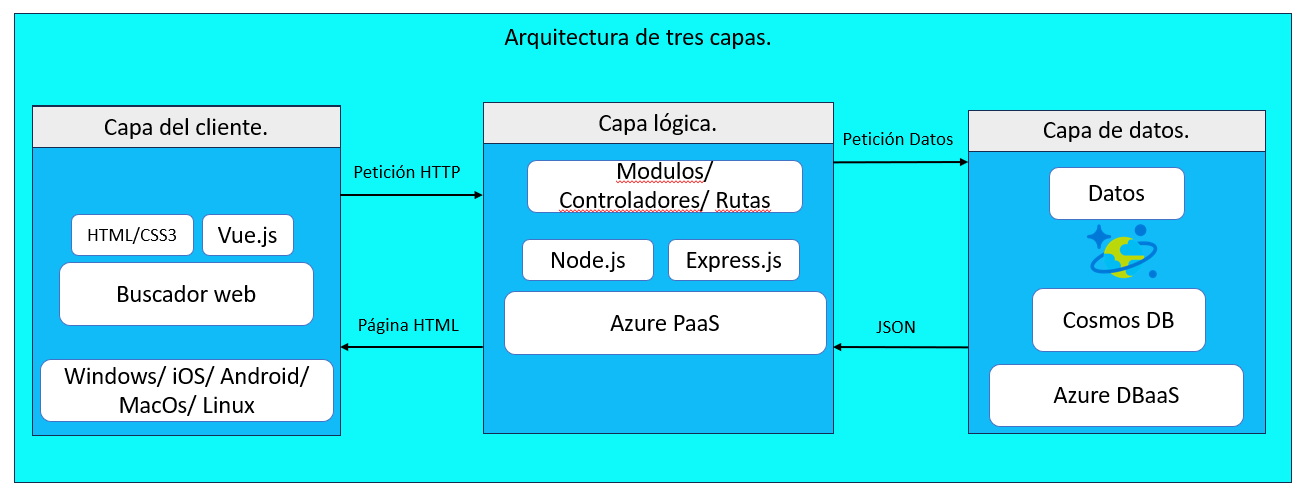
\includegraphics[width=.6\textwidth]{images/arqui/3capas}}
		\caption{Arquitectura del sistema.}
		\label{fig:arquitectura}
	\end{center}
\end{figure}

En la figura~\ref{fig:arquitectura} se describe la estructura del sistema.
